\section{Abstract}
In diesem Versuch geht es um die Positronen Emissions Tomographie (PET). Es ist ein bildgebenes Verfahren, das in der Medizin zur Tumorerkennung eingesetzt wird. Dabei wird dem Patienten ein radioaktives Material verabreicht, welches mit Detektoren, die um den Patienten in einem Kreis verteilt sind, näher untersucht werden kann. Da sich das radioaktive Material im Tumor anreichert, da es dort zu erhöhtem Stoffwechsel kommt, kann damit auch die genaue Postion des Tumors bestimmt werden.

Im letzten Teil wurde die Auflösung des Aufbaus bestimmt. Zwei Quellen können demnach nur unterschieden werden, wenn sie mindestens $\SI{63,3\pm34,0}{mm}$ voneinander entfernt stehen. Sowohl der Wert als auch die Unsicherheit sind sehr hoch, was vor allem am unzureichenden Versuchsaufbau und Rekonstruktionsalgorithmus liegt.

\section{Theorie}
\subsection{$\beta^{+}$-Zerfall}
Die PET basiert auf den $\beta^{+}$-Zerfall bei dem ein Proton im Kern in ein Neutron zerfällt und dabei ein Positron und ein Neutrino emittiert.

\begin{equation}
	^{A}_{Z}X \rightarrow ^{A}_{Z-1}Y + e^{+} + \nu_{e}
\end{equation}
Wenn das emittierte Positron auf ein Elektron im umgebenen Material trifft, kann sich ein sogenanntes Positronium bilden. Ein Positronium ist ein gebundener Zustand zwischen einem Elektron und einem Positron, wobei sich diese um ihren gemeinsamen Schwerpunkt bewegen. Hierbei gibt es zwei verschiedene Spin-Zustände, den Singulett (Parapositronium)- und Triplett-Zustand (Orthopositronium). Der Singulett-Zustand bedeutet, dass der Spin des Elektrons und des Positrons antiparallel zueinander ausgerichtet sind, während beim Triplett-Zustand sie genau parallel zueinander sind. Für den Versuch relevant ist nur der Singuelett-Zustand, da dieser, wegen Impuls- und Drehimpulserhaltung (Spin), nur in zwei oder mehrfache von zwei Photonen zerfallen kann. Im Normalfall zerfällt das Positronium allerdings in genau zwei Photonen, die jeweils die Energie von 511 keV besitzen und in genau gegensätzliche Richtungen emittiert werden. Der Triplett-Zustand kann nur in mindestens drei Photonen zerfallen, weshalb es eine deutlich längere Lebenszeit hat und nicht ohne weiteres ausgewertet werden kann. Allerdings kommt es durch die längere Lebenszeit vor, dass es zu Wechselwirkungen mit der Umgebung kommt und das Orthopositronium sich in ein Parapositronium umwandelt.

\subsection{Wechselwirkung mit Photonen und Materie}
Für die PET Messung müssen die zwei 511 keV Photonen in den Detektoren nachgewiesen werden. Damit das passieren kann, muss die Gamma-Strahlung in den Detektoren, in diesem Fall ein BGO Szintillationskristall, erfasst werden. Dabei gibt es drei verschiedene relevante Arten der Wechselwirkung.

\begin{itemize}  
	\item Photoeffekt: Beim Photoeffekt interagiert ein Photon mit einem Hüllenelektron, sodass die gesamte Energie des Photons auf  das absorbierende Material übertragen wird. Die Wahrscheinlichkeit, dass dies auftritt, geht mit $Z^{5}$/$E_{\gamma}^{3}$. Das bedeutet, dass die Wahrscheinlichkeit mit steigender Energie abnimmt, allerdings mit höhere Ladungszahl stark steigt.
	\item Compton Streuung: Bei der Comptonstreuung streut ein Photon an einem quasi freien Elektron. In Wirklichkeit sind die Elektronen zwar gebunden, was aber besonders bei äußeren Elektronen vernachlässigt werden kann. Die übertragende Energie beträgt:
	\begin{equation}
	E_e = E_\gamma \left( 1-\frac{1}{1 + \frac{E_\gamma}{m_ec^2}\left( 1-\cos\left(\theta\right)\right)}\right)
	\label{eq:compton}
	\end{equation}
	Die übertragende Energie hängt also nur vom Winkel zwischen Photon und Elektron ab. Wird der Winkel größer so nimmt auch die übertragende Energie zu, bis zu einem Maximum bei $\theta =$ 180°. 
	\item Paarbildung: Bei der Paarbildung zerfällt ein Photon in ein Elektron und ein Proton. Das kann allerdings wegen der Ruhemasse der beiden Teilchen nur ab der Grenzenergie von $E_{\gamma} = 1022$ keV geschehen und ist in diesem Fall nur für den Zerfall von Neon in den Grundzustand relevant.
\end{itemize}
In \cref{Wechselwirkung} ist Beispielhaft zu sehen, wie stark die Auswirkung der drei verschiedenen Wechselwirkungen bei verschiedenen Materialien und Energien jeweils ist.


\begin{figure}[h!]
	\centering
	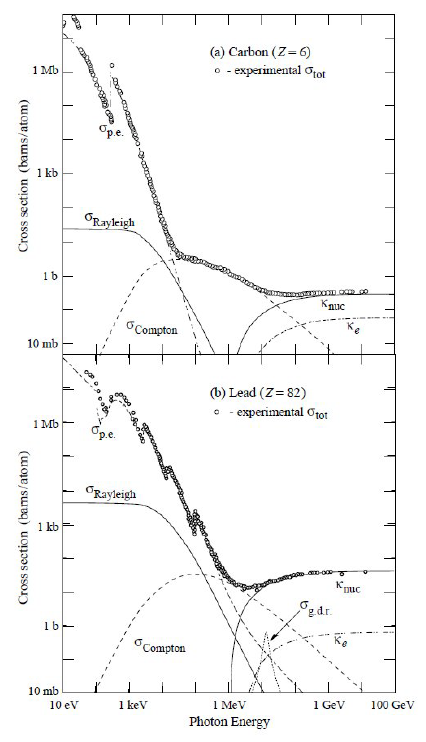
\includegraphics[width=0.5\textwidth]{Wechselwirkung.png}
	\caption{}
	\label{Wechselwirkung}
\end{figure}

\subsection{Szintillator}
Allgemein wird beim Szintillator das Material durch $\gamma$-Strahlung oder geladene Teilchen angeregt und diese deponierte Energie dann wieder als Licht emittiert. Dabei ist die Anzahl der erzeugten Photonen proportional zu der Energiemenge, die im Szintillator deponiert wurde.
Bei diesem Versuch wird ein anorganische Szintillator aus Bismutgermanat (BGO) eingesetzt. Dieser funktioniert so, dass über eine Dotierung Aktivatorzentren geschaffen werden. Über diese Aktivatorzentren läuft dann, nachdem die Elektronen über Strahlung angeregt wurden, der Abregungsprozess, sodass Photonen entstehen, die nicht mehr zur Anregung eines anderen Elektrons ausreicht. Damit ist das Material für die erzeugten Photonen transparent. Diese Photonen, die im Normalfall im UV- oder sichtbaren Bereich liegen, werden dann an einen Photomultiplier weitergegeben, von dem die Funktionsweise in \cref{Photo} zu sehen ist. 

\begin{figure}[h!]
	\centering
	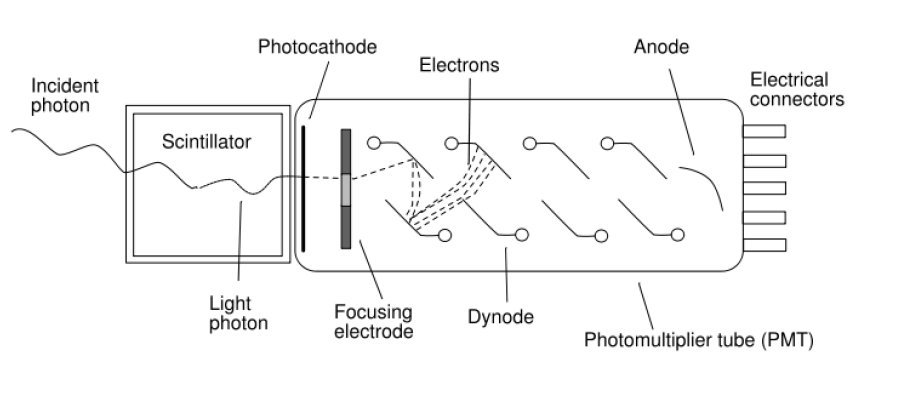
\includegraphics[width=0.9\textwidth]{Photo.png}
	\caption{Funktionsweise eines Photomultipliers}
	\label{Photo}
\end{figure}

Der elektrische Puls des Photomultipliers wird dann durch die nachgeschaltete Elektronik verstärkt und mit einem Flash Analog Digital Converter (FADC) abgetastet und digitalisiert.

\subsection{Strahlungsquelle}
Als Strahlungsquelle wird das Natrium Isotop $^{22}$Na eingesetzt. Diese Quelle beseitzt eine Halbwertszeit von 2,6 Jahren um zu $^{22}$Ne zu zerfallen. Dabei laufen 90,3\% aller Zerfälle über einen $\beta^{+}$-Zerfall un den angeregten Zustand von $^{22}$Ne, der daraufhin durch Emission eines Photons in der Grundzustand übergeht. Mit 9,64\% über einen Electron Capture Prozess. Allerdings wird dabei kein Positron freigesetzt, weshalb dieser Prozess auch nicht relevant für den versuch ist. Zuletzt kann es mit einer Wahrscheinlichkeit von 0,06\% auch zu einem direkten Übergang in den Grundzustand kommen. Für uns relevant ist also nur der indirekte $\beta^{+}$-Zerfall, bei dem zwei 511 keV Photonen durch das Positronium entstehen und ein 1275 keV Photon durch den Übergang in den Grundzustand.

\subsection{Bildrekonstruktion}
Für die Bildrekonstruktion werden nur Ereignisse untersucht, bei denen zwei Detektoren gleichzeitig ein 511 keV Photon nachweisen. Dann kann man davon ausgehen, dass es sich dabei um einen einzelnen Zerfallsprozess gehandelt hat. Es werden also nur die Ergebnisse herausgefiltert, bei denen genau dies der Fall ist. Dieses gefilterte Energiespektrum wird dann in einer 32 x 32 Matrix abgespeichert, wobei jeder Eintrag für ein Detektorpaar steht. Aus dieser Matrix kann ein Sinogramm berechnet werden, dass für die gemessenen Koinzidenzen eine Projektion mit der Formel:
\begin{equation}
	r = x \cos{\phi} + y \sin{\phi}
\end{equation}
erzeugt. Zu sehen ist das Beispielhaft in \cref{Sino} für den Eintrag zwischen Detektor 12 und 31.

\begin{figure}[h!]
	\centering
	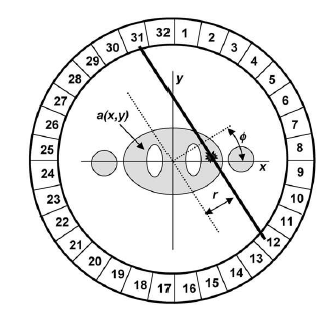
\includegraphics[width=0.9\textwidth]{Sino.png}
	\caption{Beispielbild eines Sinogramms für den Eintrag zwischen Detektor 12 und 31.}
	\label{Sino}
\end{figure}

Zur Rekonstruktion gibt es zwei grundsätzlich verschiedene Methoden zur Bildrekonstruktion. Die Erste ist die Backprojection, bei der eine Linie wie im Bild des Sinogramms gezogen wird. Jede dieser Linien hat eine bestimmte Anzahl an Koinzidenzen N. Jedem Pixel wird also gewichteter Wert $N \cdot w$ zugeordnet, wobei w beschreibt, wie lange die gezeichnete Linie durch den Pixel geht. Der Wert ist also größer, je mittiger die Linie durch den Pixel geht. Mathematisch gesehen lässt sich das Bild dann über:
\begin{equation}
	a'(x,y) = \frac{1}{N} \sum_{n = 1}^{N}s(r,\phi_{n})
\end{equation}
darstellen, wobei a'(x,y) das backprojected Bild ist. Das Problem ist allerdings, dass das Bild nur eine Näherung ist und auch Werte außerhalb der möglichen Grenze liefert weshalb besonders komplizierte Objekte nicht mehr zu erkennen sind. Allerdings kann das wirkliche Bild über eine Faltung bestimmt werden:
\begin{equation}
	a'(x,y) = a(x,y)  * \frac{1}{r}.
\end{equation}
Das Problem dabei ist allerdings, dass das direkte Ausrechnung sehr rechenintensiv und fehleranfällig ist, weshalb die filtered backprojection angewendet wird mit:
\begin{equation}
	a(x,y) = \frac{1}{N} \sum_{n = 1}^{N} s^{*}(r,\phi_{n}),
\end{equation}
wobei $s^{*}$ mit einem Fourierfilter $H(\nu) = |\nu|$ modifiziertes Sinogramm Daten sind.

Damit lässt sich die Faltung umgehen. Allerdings gibt es neben dem schon angesprochenen Filter, noch andere die versuchen statistische Fehler zu reduzieren. Diese sind in \cref{Filter} zu sehen.


\begin{figure}[h!]
	\centering
	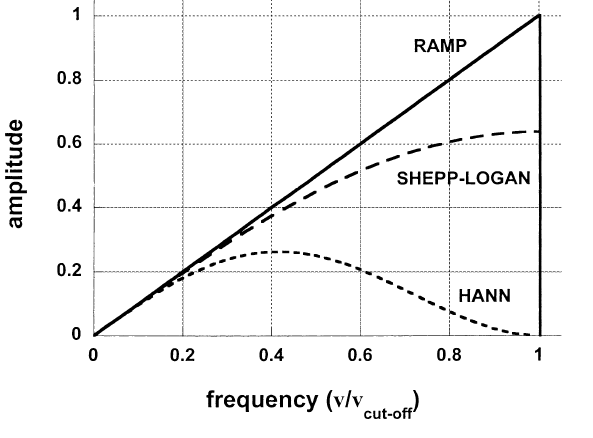
\includegraphics[width=0.9\textwidth]{Filter.png}
	\caption{Verschiedene Filter, die zur Modulation des Sinogramms benutzt werden können.}
	\label{Filter}
\end{figure}

Der andere Prozess ist ein iterativer Algorithmus, wobei zuerst ein Ausgangsbild angenommen wird, dass dann mit dem projizierten Bild verglichen wird. Dieses Bild wird daraufhin anhand der Unterschiede verändert. Dieser Vorgang wird solange wiederholt, bis ein genaues Bild errechnet wurde. Damit kann mit höherem Rechenaufwand auch ein genaueres Bild rekonstruiert werden.

\section{Methoden}
Für den Versuch musst zuerst die Hochspannung langsam hochgefahren werden. Danach mussten verschiedene Parameter des FADCs bestimmt werden. 
Daraufhin wird das grafische Interface der Datenaufnahme gestartet und nach der Einstellung der Parametern des FADCs die Integration der Signale durchgeführt. Dann werden die Einstellungen und insbesondere der Threshhold solange verändert bis das Spektrum klar erkennbar ist. In diesen Spektren sind zwei Peaks zu sehen, die nach Literaturwert bei 511 keV und 1275 keV liegen sollten. Über diese Peaks kann der Szintillator kalibriert werden, wie in \cref{Kali} zu sehen ist. Der niedrigste Peak ist dabei nicht relevant, da der von der Comptonkante stammt.
Zuletzt wird ein Energiefenster von 450-600 keV festgelegt, damit nur die relevanten 511 keV Signale aufgenommen werden. Für die Messung wird der Behälter mit der Probe auf 0° auf der darunterliegenden Skala eingestellt. Zur Simulation von 32 Detektoren werden 20 verschiedene Winkel eingestellt, sodass eine vollständige Koinzidenzmatrix erstellt werden kann. 

\begin{figure}[h!]
	\centering
	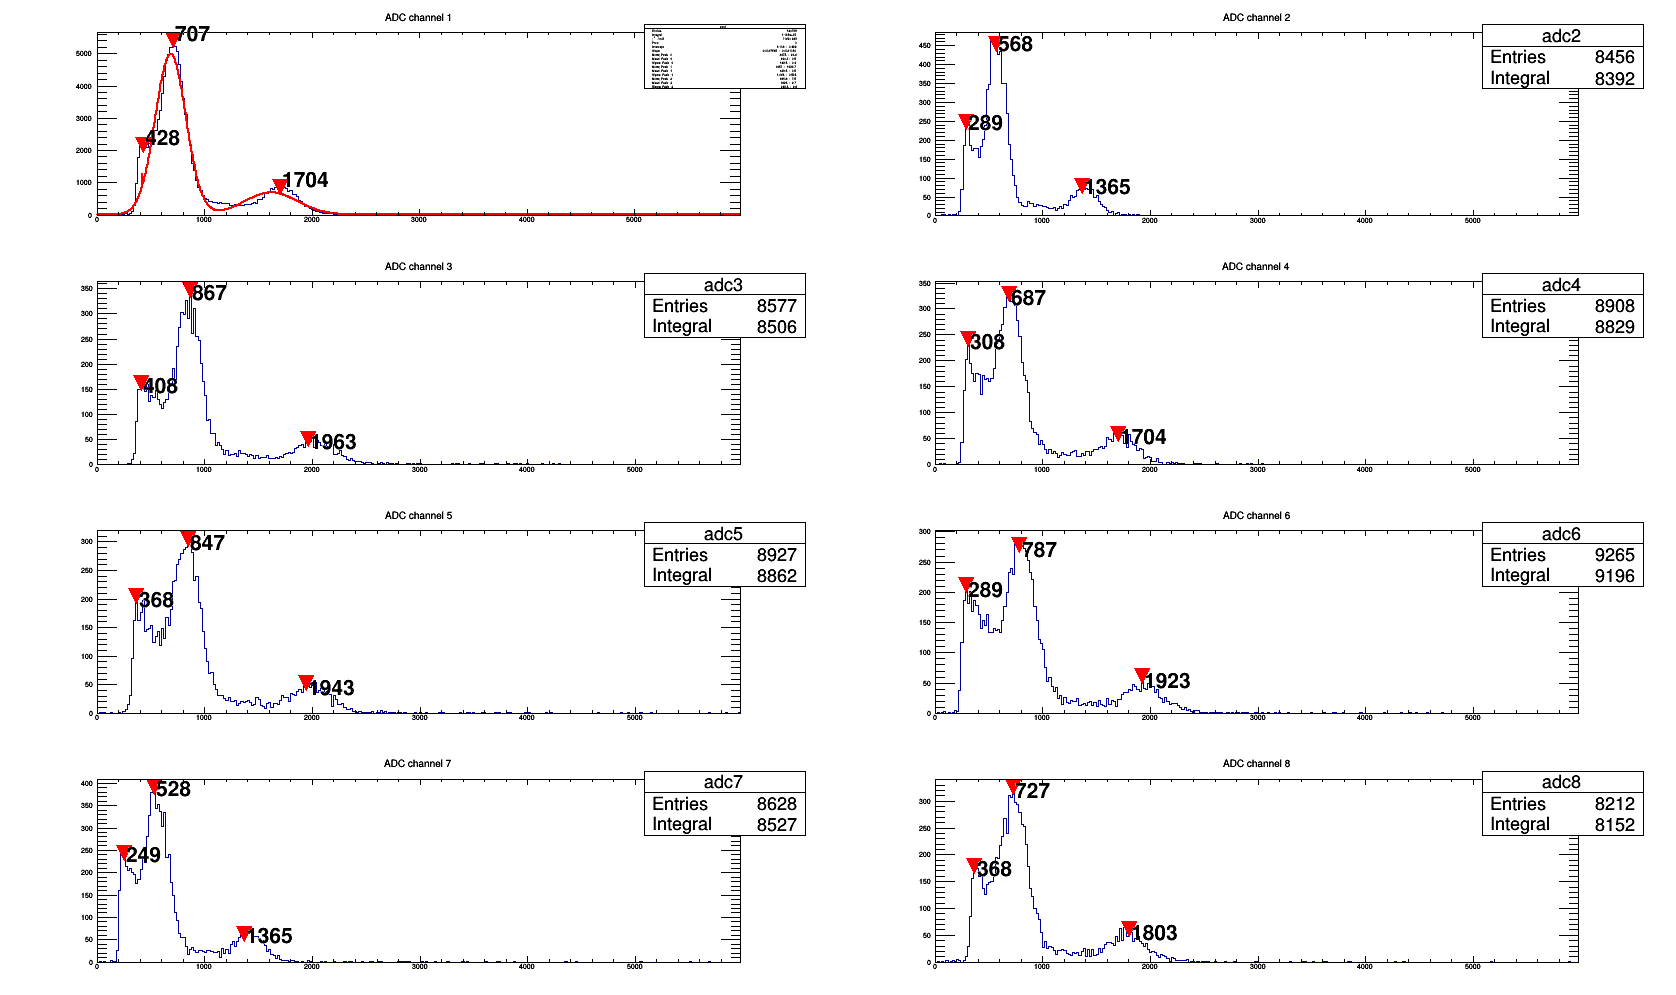
\includegraphics[width=0.9\textwidth]{Energiekalibration.png}
	\caption{Energie Spektren der acht verschiedenen Detektoren mit Peakfinder}
	\label{Kali}
\end{figure}

Die Analyse selbst erfolgt mit verschiedenen Rekonstruktionsalgorithmen, damit ein Abbild der Aktivitätsverteilung und der X-Projektion erhalten werden kann.

\section{Auswertung}
\subsection{Rekonstruktionsalgoritmen}
Zuerst wird ein 22Na-Strahler in den Koordinatenurspung des MiniPET gestellt. Dann wird durch verschiedene Rekonstruktionalgorithmen ein 2D Bild dargestellt. Durch den Maximalwert der Intensitätsverteilung wird eine Gerade durchgezogen, welche die Intensität auf die Channelnummer aufträgt. Über den zu sehenden 511 keV-Peak wird ein Gaußfit angepasst, mittels dessen die Halbwertsbreite bestimmt wird.
Es werden vier verschiedene Rekonstruktionsalgorithmen verwendet. \\
Pixel Driven Bakprojektion \\
filtered Backprojection Hann \\
filtered Backprojection Shepp-Logan \\ 
filtered Backprojection Ramp \\
Für jeden Filter wird die Aktivitätsverteilung über alle verschiedenen Winkeleinstellungen gemessen. Wie oben beschrieben wurden danach die Gaußfits erstellt.
Diese sind in \cref{ooo},\cref{ooh},\cref{oos} und \cref{oor} zu sehen. Die jeweiligen Werte und Unsicherheiten ergeben sich aus den Fits. Die Halbwertsbreite muss über ($FWHM = 2,35\sigma$) zu berechnen. Diese sind in \cref{oot} berechnet worden.
\begin{figure}[h!]
	\centering
	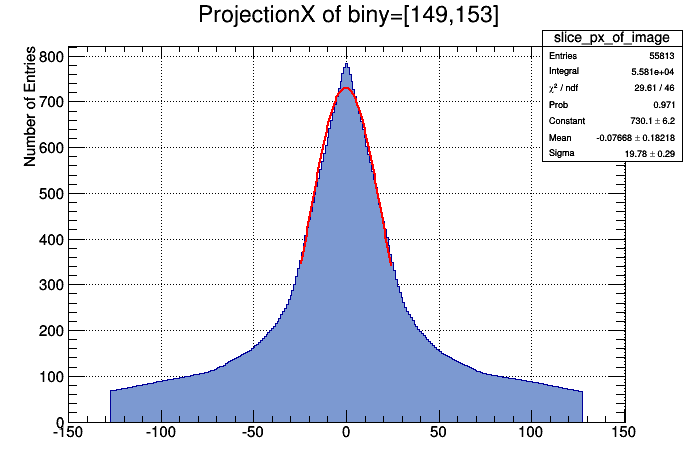
\includegraphics[width=0.9\textwidth]{Ohne-Filter.png}
	\caption{Hier wurde der Pixel Driven Backprojektion Rekonstruktionsalgorithmus benutzt. Das maximum liegt bei $-0,08 \pm 0,2$ und die Standartabweichung beträgt $19,8 \pm 0,3$.}
	\label{ooo}
\end{figure}
\begin{figure}[h!]
	\centering
	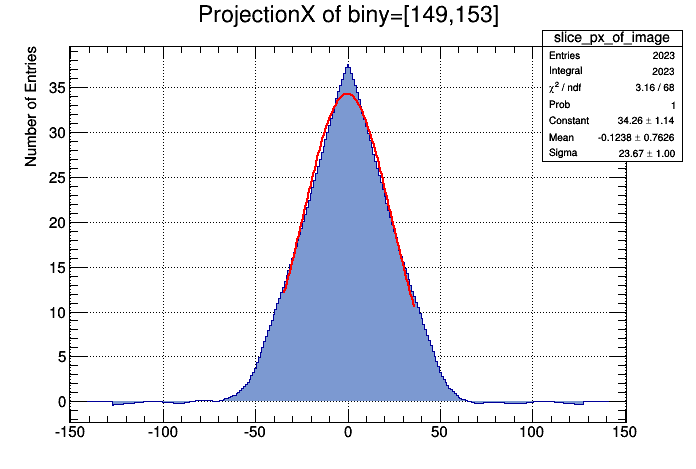
\includegraphics[width=0.9\textwidth]{Hann-Filter.png}
	\caption{Hier wurde der filtered Backprojection Hann Rekonstruktionsalgorithmus benutzt. Das maximum liegt bei $-0,12 \pm 0,8$ und die Standartabweichung beträgt $23,7 \pm 1$.}
	\label{ooh}
\end{figure}
\begin{figure}[h!]
	\centering
	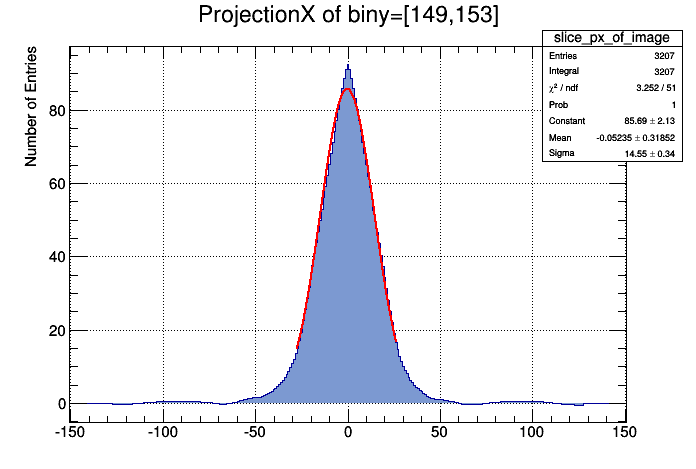
\includegraphics[width=0.9\textwidth]{Shepp-Logan-Filter.png}
	\caption{Hier wurde der filtered Backprojection Shepp-Logan  Rekonstruktionsalgorithmus benutzt. Das maximum liegt bei $-0,05 \pm 0,3$ und die Standartabweichung beträgt $14,6 \pm 0,3$.}
	\label{oos}
\end{figure}
\begin{figure}[h!]
	\centering
	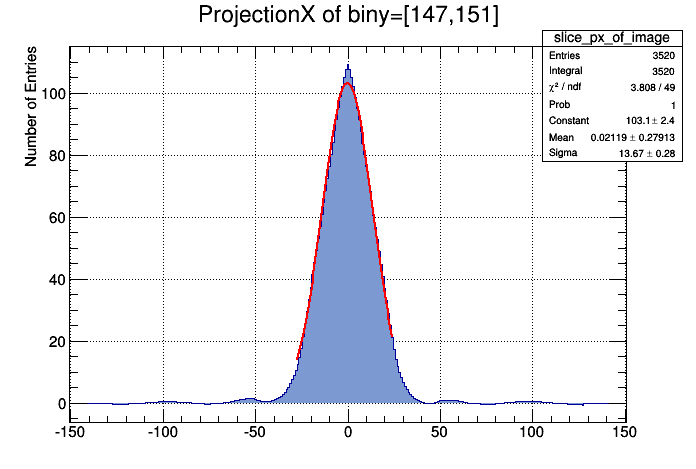
\includegraphics[width=0.9\textwidth]{Ramp-Filter.png}
	\caption{Hier wurde der filtered Backprojection Ramp Rekonstruktionsalgorithmus benutzt. Das maximum liegt bei $-0,02 \pm 0,3$ und die Standartabweichung beträgt $13,7 \pm 0,3$.}
	\label{oor}
\end{figure}
Werden die Halbwertsbreiten der verschiedenen Rekonstruktionsalgorithmen miteinander verglichen fällt auf, dass die Halbwertsbreiten von filtered backprojection Shepp-Logan und filtered backprojektion Ramp deutlich genauer sind, als die der anderen beiden.
Dabei ist der filtered backprojektion Ramp ein wenig genauer als filtered backprojection Shepp-Logan. Der filtered backprojection Hann zeigt hingegen  den breitesten Peak, mt höchster Halbwertszeit.
Ein weiterer interessanter Vergleichspunkt ist die Anzahl der Detektionen. Der pixel driven backprojection besitzt, wie in \cref{ooo} zu sehen ist, mit großen Abstand die meisten Einträge. Der Peak ist jedoch nicht am schärfsten. Es ist zu beobachten, dass dieser Rekonstruktionsalgorithmus ein Untergrund mit detektiert hat, da sich der Graf an den Rändern mehr verläuft. Ebenfalls kann hier ein Untrgrund erkannt werden. Dieses Verhalten ist bei den anderen Algorithmen nicht vorhanden.
\begin{tabular}{|c|c|c|c|}
	\hline 
	Algorithmus & Sigma & FWHM (keV) & Unsicherheiten FWHM (keV) \\ 
	\hline 
	pixel driven backprojection & 19,8 & 46,5 & 0,3 \\ 
	\hline 
	filtered backprojection Hann & 23,0 & 54 & 1  \\ 
	\hline 
	filtered backprojection Shepp-Logan & 14,4 & 33,8 & 0,3 \\ 
	\hline 
	filtered backprojektion Ramp & 13,7 & 32,2 & 0,3 \\ 
	\hline 
	\label{oot}
\end{tabular} 
Anhand der Halbwertsbreiten ist zu erkennen, dass der filtered backprojektion Ramp Algorithmus der präziseste Algorithmus ist. Somit wird die Positionsbestimmung im weiteren Fall mit Hilfe des filtered backprojektion Ramp Algorithmus berechnet.
Das iterative Rekonstruktionsverfahren wurde in diesem Bericht weggelassen.

\subsection{Positionsbestimmung}
Bei den rekonstruierten Bildern ist die Intensität in einem Graphen von 300x300 Pixeln gegeben. Somit muss die pixelabhängigkeit in den Gaphen erst in Positionen im Raum umgerechnet werden. Dazu werden weitere Messungen mit dem filtered backprojektion Ramp Algorithmus durchgeführt an  verschiedenen Stellen im Raum. Mit diesen Messungen kann eine Kalibration im Raum vorgenommen werden. In \cref{oop} ist die Position der Gaußmaxima gegen die tatsächliche Position aufgetragen.
\begin{figure}[h!]
	\centering
	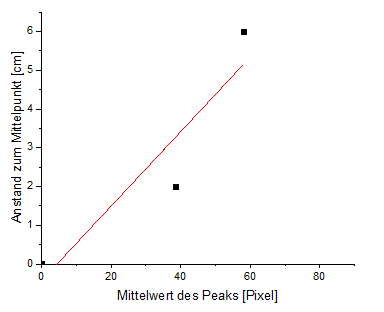
\includegraphics[width=0.9\textwidth]{Position.png}
	\caption{Die Parameter der Geraden sind für den y-Achsenabschnitt(y) $y = -0,4 \pm 1,5$ und für die Steigung(m) $m = 0,10 \pm 0,03 $}
	\label{oop}
\end{figure}
Aus der Fitgeraden lässt sich der Umrechnungsfaktor vom Ort(x) in cm und der Bildposition(xp) in Pixeln bestimmen.
\begin{align}
	x = m \cdot xp =  (0,10 \pm 0,03)\frac{cm}{Pixel} xp
\end{align}
Mittels Fehlerfortpflanzung lässt sich der Fehler für die Positionsbestimmung errechnen.
Hier werden zwei Fehlerquellen angenommen. Einmal wird der Fehler aus dem filtered backprojektion Ramp Algorithmus genommen und einmal der Fehler der Fitgeraden.
\begin{align}
	u(x) &= \sqrt{(xpu(m))^2 + (m\sigma)^2} &= 2,6cm
\end{align}
da der Fehler von der Position xp abhängig ist, wird der mittlere Radius (xp = 75) für die Fehlerabschätzung verwendet

\subsection{Auflösung}
Zuletzt wurde noch die Auflösung des Versuchaufbaus bestimmt. Hierfür wurden zwei $^12$Na-Quellen verwendet. Diese wurden mit verschiedenen Abständen zueinander im Detektor positioniert. Anschließend wurde mit dem Ramp-Rekonstruktionsalgorithmus der wahrscheinliche Aufenthaltsort beider Quellen bestimmt. Dieser wurde anschließend eindimensional mit einem Gauss-Fit genähert. Dazu wurde im rekonstruierten Bild nur die Informationen entlang der x-Achse verwendet. Diese Fits sind in \cref{abstand} dargestellt.

\begin{figure}[h]
	\centering
	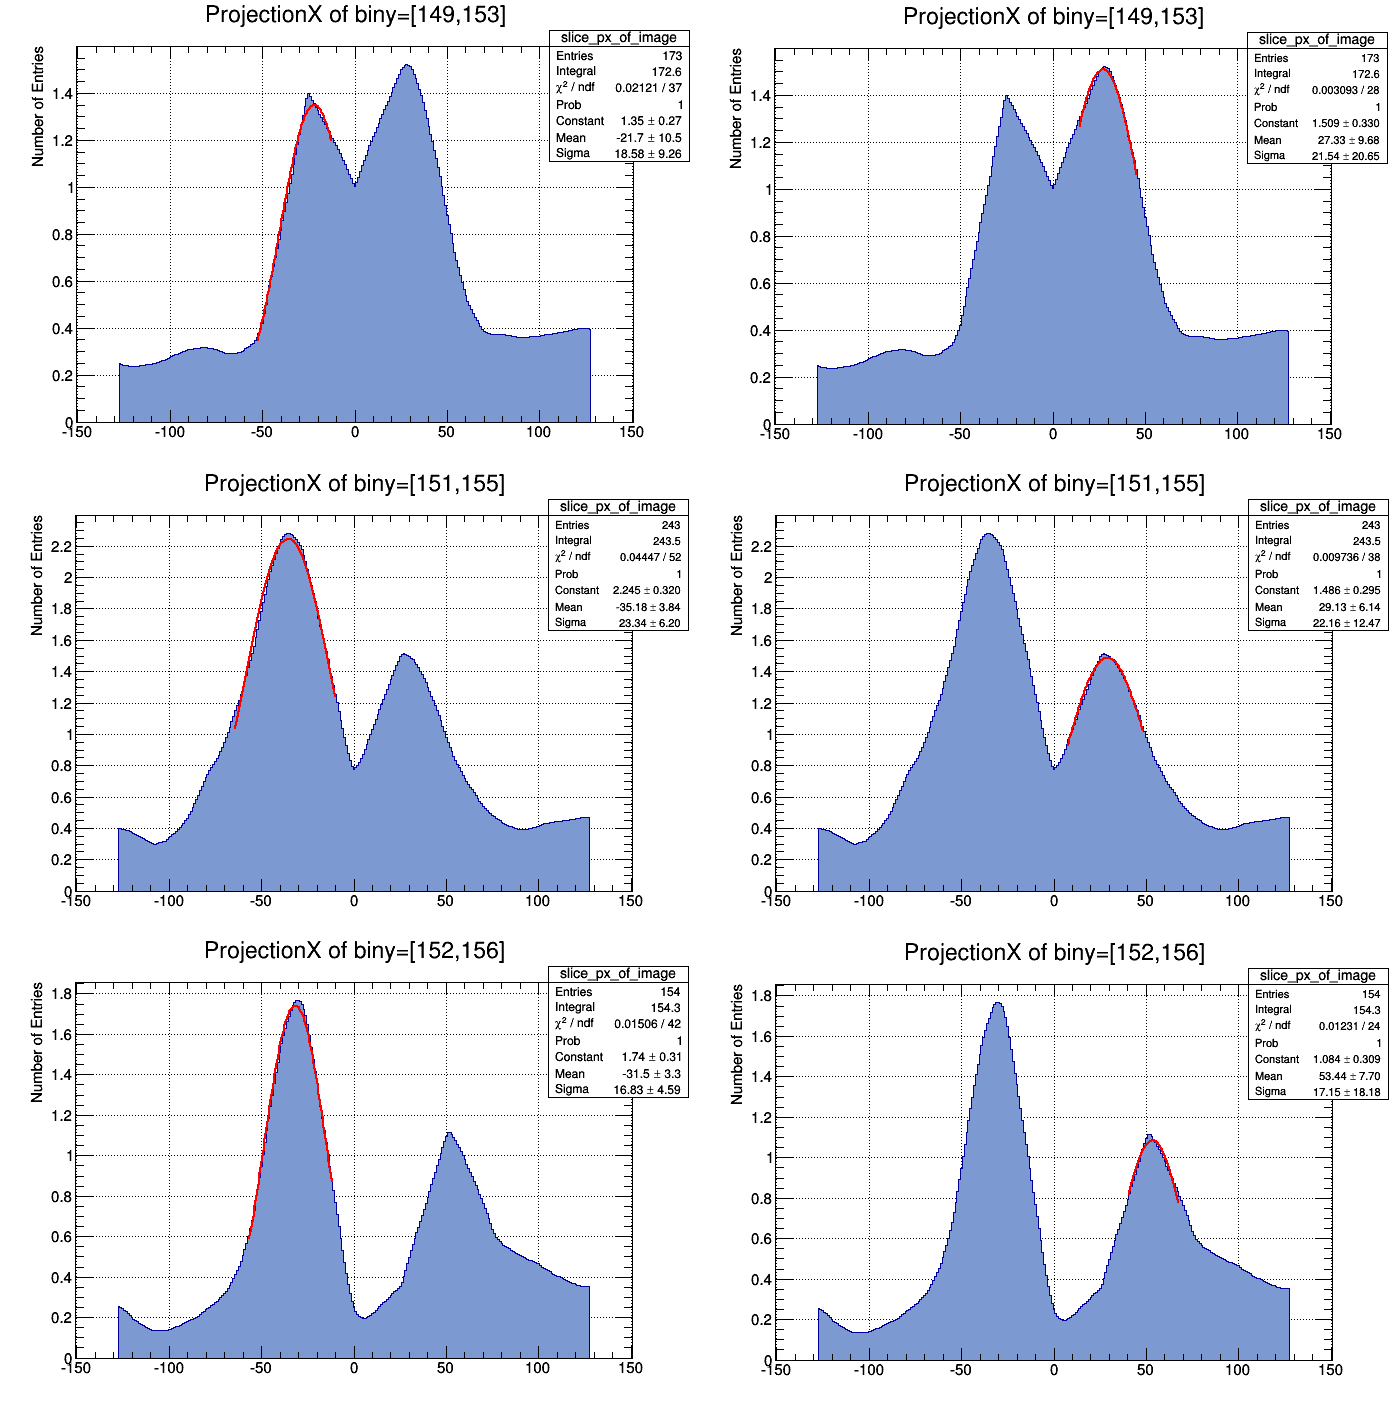
\includegraphics[width=0.9\textwidth]{abstand_alle.png}
	\caption{Jeweils zwei Fits für alle verschiedenen Abstände der Quellen}
	\label{abstand}
\end{figure}

Nun wurde für drei verschiedene Abstände (60, 80 und \SI{100}{mm}) der gemessene Abstand zwischen den Punkten, an denen die Gaussverteilung jeweils auf die Hälfte abgefallen ist, bestimmt. Die FWHM wurden mit $FWHM = 2\sqrt{2\ln(2)}$ berechnet. Diese Werte wurden anschließend in \cref{abstand_fit} eingetragen.

\begin{figure}[h]
	\centering
	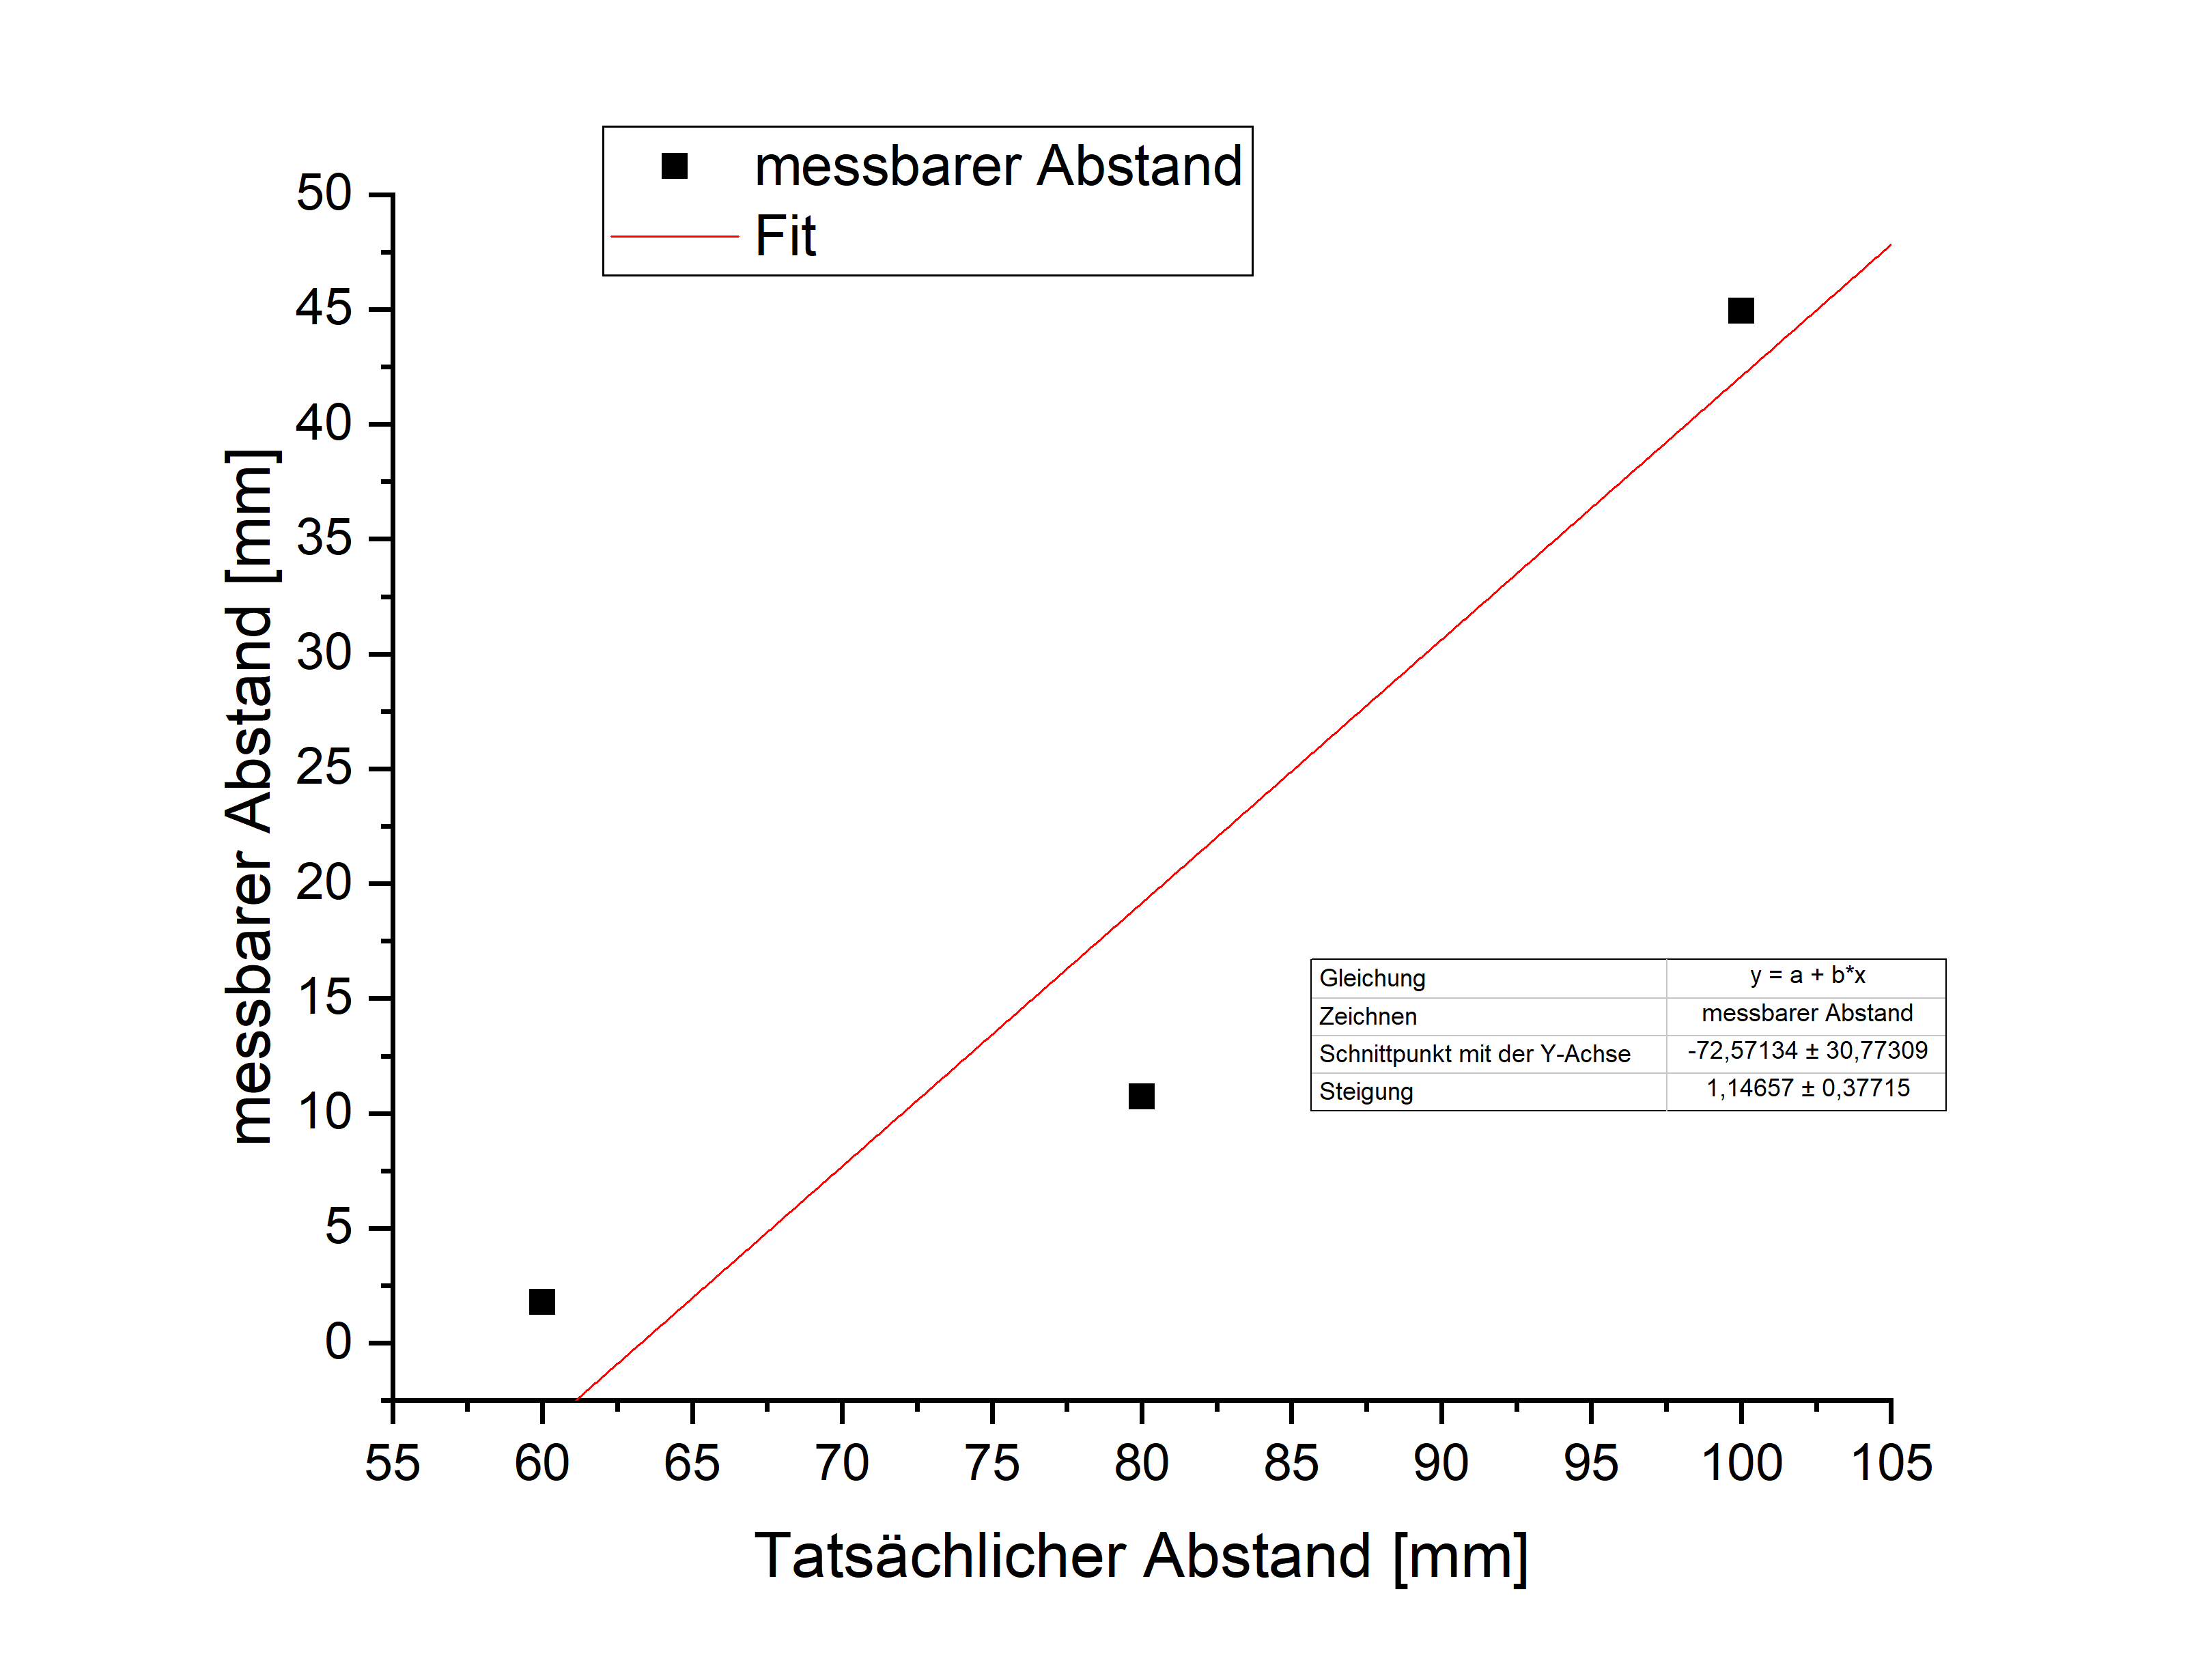
\includegraphics[width=0.9\textwidth]{abstand_fit.png}
	\caption{Der Abstand zwischen den zueinanderzeigenden FWHM der Gaussfits, aufgetragen gegen den tatsächlichen Abstand zwischen den beiden Quellen.}
	\label{abstand_fit}
\end{figure}

Unterschieden werden können Quellen nach dieser Definition, solange sich die FWHM der beiden Peaks nicht überschneiden. Die Nullstelle des linearen Fits zeigt nun an, bis zu welchem Abstand die beiden Quellen unterschieden werden können. Der gesuchte Wert beträgt $\SI{63,3\pm34,0}{mm}$. Zwei Quellen können also, wenn sie näher aneinander positioniert werden, nicht unterschieden werden. Sowohl der berechnete Wert als auch die dazugehörige Unsicherheit liegen im Zentimeterbereich. Damit ist die hier verwendete Kombination von Aufbau und Rekombinationsalgorithmus nicht für den eigentlichen Zweck von PET, der genauen Lokalisierung von Tumoren, geeignet. Das liegt zum Beispiel daran, dass hier nur acht Detektoren verwendet werden, die im Kreis um die Quelle verschoben werden. Außerdem sind alle hier verwendeten Rekonstruktionsalgorithmen immer noch deutlich schlechter als die iterative Methode. Die Ungenauigkeit der Daten zeigt sich auch am Wert für den messbaren Abstand bei 6cm Abstand zwischen den Quellen. Laut Bild (\cref{abstand}) und Nullstelle der Fitgerade sollten die beiden Quellen in diesem Fall nicht mehr unterscheidbar sein, laut Rechnung (in \cref{abstand_fit} eingetragener Wert) sind sie allerdings noch unterscheidbar. Das liegt vor allem an den vom Programm erstellten Gauss-Fits, die die Messwerte unzureichend darstellen.